\documentclass[UTF8]{ctexart}
\usepackage{subfigure}
\usepackage{caption}
\usepackage{amsmath,bm}
\usepackage{amssymb}
\usepackage{pifont}
\usepackage{geometry}
\usepackage{graphicx}
\usepackage{gensymb}
\usepackage{wrapfig}
\usepackage{titlesec}
\usepackage{float}
\usepackage{diagbox}
\usepackage{fancyhdr}
\usepackage{color}
\usepackage{bm}
\usepackage{ulem}
\usepackage{CJKulem}
\pagestyle{plain}
\geometry{a4paper,scale=0.8}
\CTEXsetup[format+={\raggedright}]{section} 
\title{固物2014期中A卷}
\author{Deschain}
\titlespacing*{\section}
{0pt}{0pt}{0pt}
\titlespacing*{\subsection}
{0pt}{0pt}{0pt}
\titlespacing*{\paragraph}
{0pt}{0pt}{0pt}
\titlespacing*{\subparagraph}
{0pt}{0pt}{0pt}
\titleformat*{\section}{\normalsize}
\begin{document}
\maketitle
\section*{\bfseries 物理常数}
\begin{equation*}
    \begin{aligned}
        & k_B=1.381\times10^{-23}J\cdot K^{-1}\quad\hbar=1.054\times10^{-34}J\cdot s\quad 
        q=1.602\times10^{-19}C\quad m=9.109\times10^{-31}kg\\
        & N_A=6.022\times10^{23}
    \end{aligned}
\end{equation*}
\section*{\bfseries 1.填空题(每空1分,共30分)}
(1)GaAs的晶体结构是\uline{\makebox[4em]{}}结构,其布拉菲格子是\uline{\makebox[6em]{}}
格子。\\
(2)碱金属晶体是体心立方晶格,其倒格子为\uline{\makebox[6em]{}}格子。若倒格子基矢为$\vec\beta_1,
\vec\beta_2,\vec\beta_3$,则碱金属晶体晶面指数为(231)的晶面族的面间距可表示为\uline{\makebox[10em]{}}。
假设碱金属的晶格常数为$a$,则其电子浓度为\uline{\makebox[2em]{}}。\\
(3)假设Si的晶格常数为$a$,则其布拉菲格子原胞的体积为\uline{\makebox[2em]{}},第一布里渊区的体积为
\uline{\makebox[3em]{}}。\\
(4)晶体中的缺陷按其几何类型可以分为\uline{\makebox[2em]{}}缺陷、线缺陷和\uline{\makebox[2em]{}}
缺陷。其中线缺陷又分为\uline{\makebox[3em]{}}位错和\makebox[2em]{}位错。\\
(5)原子的结合中,吸引作用主要来自于异性电荷之间的\uline{\makebox[3em]{}}作用,而排斥作用来自于同性电荷
之间的\uline{\makebox[3em]{}}作用以及\uline{\makebox[7em]{}}原理引起的排斥。一般固体的结合可以概括
为四种基本形式,除了离子性结合之外,还包括\uline{\makebox[4em]{}}结合、\uline{\makebox[4em]{}}结合
和\uline{\makebox[9em]{}}结合。金刚石材料中C-C键结合的方式是典型的\uline{\makebox[3em]{}}结合,其
电离度为\uline{\makebox[2em]{}}。\\
(6)假设金属晶体的总体积为$V$,则$k$空间的点阵密度为\uline{\makebox[3em]{}}。能量标度下电子的能态密度会
随着能量的增大而\uline{\makebox[3em]{}}。\\
(7)两块同种原子组成的金属晶体,体积分别为$V_1$和$V_2$,且$V_1>V_2$,则自由电子的数目$N_1$
\uline{\makebox[2em]{}}$N_2$,费米能级$E_{F1}$\uline{\makebox[2em]{}}$E_{F2}$。(填$>,<,=$)\\
(8)布洛赫能带理论相比索末菲自由电子模型,主要是考虑了晶体中的\uline{\makebox[7em]{}}对电子运动的影响。\\
(原图缺失)\\
\section*{\bfseries 2.简答题(每题5分,共20分)}
(1)请简述晶体、非晶体和准晶体之间的区别。\\
(2)请说明空穴的物理意义。\\
(3)请描述周期性边界(波恩-卡曼)条件并说明其在什么条件下适用。\\
(4)请用能带理论简述导体、绝缘体和半导体的区别。\\
\section*{\bfseries 3.(8分)如图所示,是一个体心立方晶格的单胞,其晶格常数为$a$,A和B都是各自边矢量的中点。}
(1)写出OAB晶面的密勒指数。\\
(2)求OAB晶面的面间距。\\
\begin{figure}[H]
    \centering
    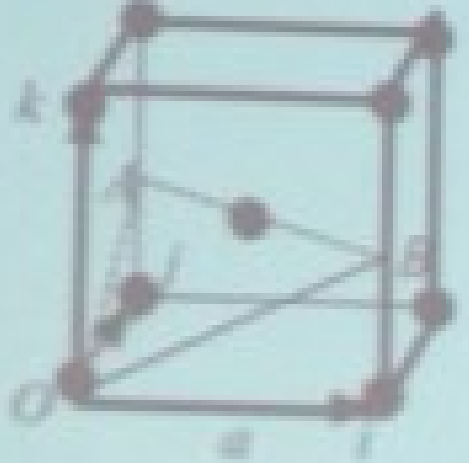
\includegraphics[width=4cm,height=4cm]{3.png}
\end{figure}
\section*{\bfseries 4.(6分)相距为$r$的两原子,相互作用势能可以表示为$u(r)=u_0[(\frac{\sigma}{r})^m-
(\frac{\sigma}{r})^n]$,分别求出势能最小值和吸引力最强时的距离。(原题不是m和n,但图片看不清)}
\section*{\bfseries 5.(8分)假设一个晶格常数为$a$的一维晶格中,电子能量$E(k)=E_0-2E_1cos(ka)$,其中$E_1>0$}
(1)分别求能带底和能带顶处的简约波矢和能量。\\
(2)分别求能带底和能带顶处电子的有效质量。\\
\section*{\bfseries 6.(8分)电子在一个晶格常数为$a$的一维晶体中运动。}
(1)求布里渊区边界$\frac{2\pi}{a}$处自由电子的能量。\\
(2)假设单个电子感受到的周期性势场$V(x)=-V_0cos(\frac{4\pi x}{a})cos(\frac{2\pi x}{a})$,其中$V_0>0$。采用
近自由电子近似分别求出布里渊区边界$\frac{\pi}{a},\frac{2\pi}{a},\frac{3\pi}{a}$处的能隙。\\
\section*{\bfseries 7.(20分)已知一种由同种原子组成的金属晶体。(原图缺失)}
\newpage
\section*{\bfseries 1.填空题答案}
(1)\ding{172}闪锌矿\makebox[2em]{}
\ding{173}面心立方\\
(2)\ding{172}面心立方\makebox[2em]{}
\ding{173}$\frac{2\pi}{\lVert\vec\beta_1+\vec\beta_2+\vec\beta_3\rVert}$\makebox[2em]{}
\ding{174}$\frac{2}{a^3}$\\
(3)\ding{172}$\frac{a^3}{4}$\makebox[2em]{}
\ding{173}$\frac{32\pi^3}{a^3}$\\
(4)\ding{172}点\makebox[2em]{}
\ding{173}面\makebox[2em]{}
\ding{174}刃形\makebox[2em]{}
\ding{175}螺形\\
(5)\ding{172}吸引\makebox[2em]{}
\ding{173}排斥\makebox[2em]{}
\ding{174}泡利不相容\makebox[2em]{}
\ding{175}共价\makebox[2em]{}
\ding{176}金属性\makebox[2em]{}
\ding{177}范德瓦耳斯力\makebox[2em]{}
\ding{178}共价\makebox[2em]{}
\ding{179}0\\
(6)\ding{172}$\frac{V}{8\pi^3}$\makebox[2em]{}
\ding{173}增大\\
(7)\ding{172}$>$\makebox[2em]{}
\ding{173}$=$\\
(8)\ding{172}周期性势场\\
\section*{\bfseries 2.简答题答案}
(1)\ding{172}晶体:内部原子的排列具有空间周期性。\\
\ding{173}非晶体:内部原子的排列不具有周期性。\\
\ding{174}准晶体:内部原子的排列具有旋转对称性,没有平移对称性(或具有长程取向序,无长程平移序)。\\
(2)空穴是满带缺少电子的状态,实际上描述的是满带中其他电子的运动。\\
(3)\ding{172}$\psi(x)=\psi(x+Na)$\\
\ding{173}是忽略边界影响时的边界条件。\\
(4)\ding{172}导体:价带完全填充,导带部分填充,导电性良好。\\
\ding{173}绝缘体:价带完全填充,导带是空带,并且带隙较大,不易发生跃迁,因此几乎不导电。\\
\ding{174}半导体:绝对零度时,价带完全填充,导带是空带,但是带隙较小。室温下,一部分电子可以从价带上被热激发到导带上。
导带和价带都变成部分填充,可以导电。
\section*{\bfseries 3.解答}
(1)$(11\overline{2})$\\
(2)$\frac{\sqrt{6}}{3}a$\\
\section*{\bfseries 4.解答}
设势能最小的位置为$r_1$,吸引力最强的位置为$r_2$,则
\begin{equation*}
    \begin{aligned}
        & \frac{dU}{dr}=u_0(-\frac{m\sigma^m}{r^{m+1}}+\frac{n\sigma^n}{r^{n+1}})=0,\quad
        r_1=(\frac{n}{m})^\frac{1}{n-m}\sigma\\
        & \frac{d^2U}{{dr}^2}=u_0(\frac{m(m+1)\sigma^m}{r^{m+2}}-\frac{n(n+1)\sigma^n}{r^{n+2}})=0,\quad
        r_2=(\frac{n(n+1)}{m(m+1)})^\frac{1}{n-m}\sigma\\
    \end{aligned}
\end{equation*}
\section*{\bfseries 5.解答}
(1)能带底$k=0$,能量$E(0)=E_0-2E_1$\\
能带顶$k=\frac{\pi}{a}$,能量$E(\frac{\pi}{a})=E_0+2E_1$\\
(2)$m^*=\frac{\hbar^2}{\frac{\partial^2E}{\partial k^2}}=\frac{\hbar^2}{2a^2E_1cos(ka)}$\\
能带底$m^*=\frac{\hbar^2}{2a^2E_1}$,能带顶$m^*=-\frac{\hbar^2}{2a^2E_1}$\\
\section*{\bfseries 6.解答}
(1)
\begin{equation*}
    \begin{aligned}
        & E=\frac{\hbar^2k^2}{2m}=\frac{2\hbar^2\pi^2}{ma^2}\\
    \end{aligned}
\end{equation*}
(2)
\begin{equation*}
    \begin{aligned}
        & V(x)=-\frac{V_0}{4}(e^{i\frac{6\pi}{a}x}+e^{i\frac{2\pi}{a}x}+e^{-i\frac{2\pi}{a}x}+e^{-i\frac{6\pi}{a}x})\\
        & V_{\pm1}=-\frac{V_0}{4},\quad V_{\pm3}=-\frac{V_0}{4}\\
    \end{aligned}
\end{equation*}
$\frac{\pi}{a}$处能隙为$\frac{V_0}{2}$,$\frac{2\pi}{a}$处能隙为$0$,$\frac{3\pi}{a}$处能隙为$\frac{V_0}{2}$。
\end{document}